
\chapter{Differentiating between BPMN, CMMN and DMN}
\label{chapter:indicators}

\section{BPMN and routine processes}
Creating business process diagrams nowadays almost seems to be intuitive. This results from a broad background of routine process modeling incorporating the rise and fall of BPR, ARIS and its EPCs and many more routine process modeling languages. Altogether, they formed the current understanding of business process management and modeling. 
Since BPMN is a broadly adopted modeling language and a standard that shaped the industry, users might be mislead when to use BPMN correctly. In this chapter, a definition of requirements and indicators will be provided for the correct use case scenario identification in terms of BPMN as well as a short introduction to the model. 

\begin{sidewaysfigure}
	\caption{A small BPMN example: the application process for study programs.}
	\label{fig:BPMNex}
	\centering
	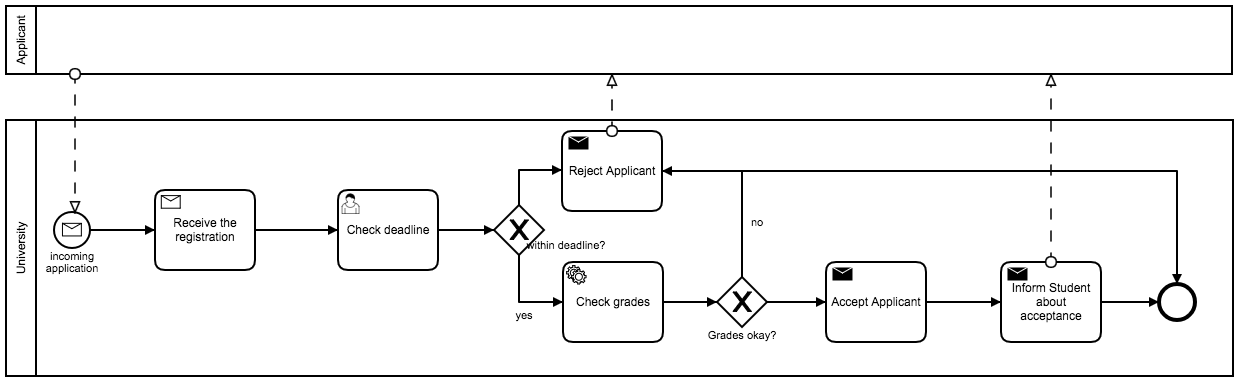
\includegraphics[scale=0.5]{../figures/differentiating/BPMN_Example_Student_Application.png} 
\end{sidewaysfigure}

Business Process Model and Notation incorporates \textit{Business Process}, which has been defined and redefined many times by today. For this thesis, we use the OMG's definition of business processes: 
\begin{quote}
Business Processes: business plans include Courses of Action - what the enterprise has to do to achieve its Ends - transformed into Business Processes that ecnompass activities, sequencing, dependencies, interactions, triggering by business events, etc. \cite{bmm2015}
\end{quote}

Business processes are ways to achieve goals, to align activities along them and to define interactions, decisions and events. This definition basically incorporates all the core elements of BPMN: Activities, paths, swimlanes (for responsibilities), decisions and events. To recap the notation of BPMN, a small example is shown in figure \ref{fig:BPMNex}. 
In this model, the application process for a student program is shown, which consists of tasks such as \textit{Receive the registration} or \textit{Check deadline}. Tasks can be precised as \textit{Manual tasks}, \textit{Send / Receive Tasks} and have assignees, as shown in \textit{Check deadline}. In current Workflowmanagementsystems, this workflow model can be fully automated and the assignee is presented its tasks when they are instantiated, e.g. when an application form was received. BPMN models have a starting and an end point which can also be events. In our example, the starting point is a \textit{Message Event}, that indicates the process has started due to a received message. 
Decisions are a major concern in every control flow oriented graph and BPMN models usually consist of several decision points. They are notated as diamond-shaped \textit{Gateways}, either empty or with a special symbol inside. Each symbol stands either for \textit{AND}, \textit{OR}, \textit{XOR} or \textit{COMPLEX}. Gateways direct the control flow depending on the decision logic prescribed. In our example, a \textit{XOR} Gateway controls the workflow into either the direction of acceptance or the opposite one, depending on what date the applicant's form was submitted. Additionally, the communication between the workflow's two participants is notated as so called \textit{Pools}, which can be divided into \textit{Swimlanes}. Each pool is a communication partner and a swimlane indicates different responsibilities such as departments. If a pool is not filled with BPMN elements, the communication partner is out of scope of the modeler and the processes cannot be modeled. These pools are \textit{Black boxes}. 

As we see in the example, the process is well-structured and has no room for creative decisions or even discussions at run-time. The only way the process can differ, is human intervention or changing the process at design-time. The former is equal to not executing the process in the intended way and the latter is bad for processes in volatile environments. BPMN is suited for a limited variety of processes, foremost business processes. The OMG's specification excludes specifically the following \cite{BPMNspec}: 

\begin{quote}

\begin{itemize}
\item Definition of organizational models and resources,
\item Modeling of functional breakdowns,
\item Data and information models,
\item Modeling of strategy,
\item Business rules models
\end{itemize}

\end{quote}

%Although excluded, data and information can be modeled by artifacts. It's not like an \textit{Unified Modeling Language} (UML) model where classes and inheritance is mapped, but it is useful to handle forms and different kind of documents which need to be passed along the tasks. 
%For business rules, this is also applicable. BPMN contains a special form of tasks called \textit{Business Rule Task}, which "[...] provides a mechanism for the Process to provide input to a Business Rules Engine and to get the output of calculations that the Business Rules Engine might provide" \cite{BPMNspec}. Business Rule Tasks are predestined for small spreadsheets fed injected into a business rule engine, which is usually a Java class. It is easy to use and implement, since the Business Analyst files a spreadsheet and the developer uses the CSV-file to implement the business rule engine. This procedure, however, works only at design-time and not at run-time, which is a downside being discussed in a subsequent section about DMN. 

Furthermore, the OMG's specification not only provides exclusions such as the ones mentioned above, but it helps to indicate the correct usage of BPMN. Derived from the background chapter \ref{chapter:background} and the example above, the following indicators (table \ref{tab:bpmnIndicatorsTable}) serve as a guidance for modelers to identify when to use BPMN correctly. 

% Please add the following required packages to your document preamble:
% \usepackage{booktabs}
% \usepackage{graphicx}
\begin{table}[]
\centering
\caption{BPMN indicators.}
\label{tab:bpmnIndicatorsTable}
\resizebox{\textwidth}{!}{%
\begin{tabular}{@{}ll@{}}
\toprule
Indicators                   & BPMN                                                                                                                                                                         \\ \midrule
General                      & \begin{tabular}[c]{@{}l@{}}Predefined sequences of activities with decisions (gateways) to direct the \\ sequence along the alternative paths or for iterations\end{tabular} \\
Type of process              & \begin{tabular}[c]{@{}l@{}}Predefined, fully specified, repeatable, business process, \\ control flow oriented\end{tabular}                                                  \\
Type of work                 & Routine work with possible automation                                                                                                                                        \\
Type of decisions            & Simple, driven by rules or events                                                                                                                                            \\
Control flow                 & Strict and necessary                                                                                                                                                         \\
Intervention at run-time     & no                                                                                                                                                                           \\
Typical application          & Value-added chain processes, workflows across companies, departments etc.                                                                                                    \\
Key question before modeling & \begin{tabular}[c]{@{}l@{}}Does the work consist of routine elements which can \\ be optimized or even automated?\end{tabular}                                               \\ \bottomrule
\end{tabular}%
}
\end{table}

Information about processes is often stored in documents, deprecated models or held by knowledge carriers according to Dumas et al. \cite{Dumas2013}. This information needs to be extracted by the application of the so called \textit{Process Discovery}, which is in short gathering all the information in a technical or manual way before creating the models. Having this information gathered together, the key question before modeling is \textit{Does the work consist of routine elements which can be optimized or even automated?} (see \ref{tab:bpmnIndicatorsTable}). Routine processes occur regularly and their flow is "known a priori" according to \cite{Zeising_2014}. Consequently it is not intended to change the process flow during run-time, as routine are well-structured and predefined. This is a major problem for workers whose job is more based on knowledge and their experience than routine work, wherefore is Case Management and CMMN were forged and standardized. 
In our example, the decisions are simple yes or no questions. One of them, \textit{Check grades}, is a business rule task containing a small table of when a grade acceptable or must be rejected. Overall, the decisions do not require modeling any requirements or personnel apart from the assignee involved in the decision making process. Furthermore, the decisions are always stuck with rules or events that happened before. The process itself is control-flow-oriented and the control flow is necessarily strict since every candidate needs to be processes in a fair and equal manner. In the end, the process could be automated completely with the correct workflowmanagementsystem and would not need any assignee to check the deadline or the grades. 
According to the indicators, the example is modeled using the appropriate modeling language as the process was predefined and well-structured. To prove the indicators' validity, a use case example taken from the eKulturPortal GmbH \footnote{see \url{http://ekulturportal.de/}} is provided in chapter \textbf{TODO !!!!!}. 

\section{CMMN and knowledge work}